\begin{pastexam}[label={px:ncu-109-dsa-01}]{中央資工所 109 學年度 第 1 題}
（複選；每題 5 分，全對才給分，答錯倒扣 1.25 分）

Consider the graph below. Which of the following is a DFS traversal sequence starting from node 1?

\begin{center}
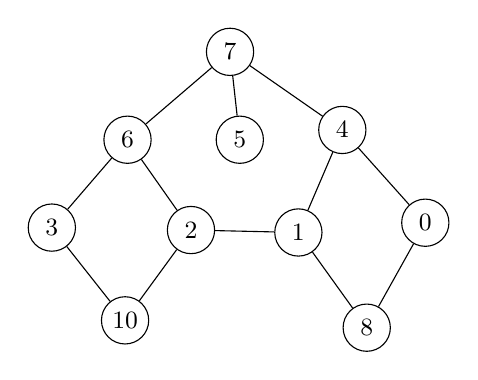
\begin{tikzpicture}[x=0.62cm,y=0.62cm,v/.style={circle,draw,inner sep=1pt,minimum size=6mm,font=\small}]
\node[v] (7) at (5.0,-0.9) {7};
\node[v] (6) at (2.9,-2.7) {6};
\node[v] (5) at (5.2,-2.7) {5};
\node[v] (4) at (7.3,-2.5) {4};
\node[v] (3) at (1.35,-4.5) {3};
\node[v] (2) at (4.2,-4.55) {2};
\node[v] (1) at (6.4,-4.6) {1};
\node[v] (0) at (9.0,-4.4) {0};
\node[v] (10) at (2.85,-6.4) {10};
\node[v] (8) at (7.8,-6.55) {8};
\draw (7)--(6) (7)--(5) (7)--(4) (6)--(3) (6)--(2) (2)--(1) (4)--(1) (4)--(0) (3)--(10) (2)--(10) (1)--(8) (0)--(8);
\end{tikzpicture}
\end{center}

(A)~1 2 6 7 4 0 8 5 3 10\\
(B)~1 8 0 4 7 5 6 3 10 2\\
(C)~1 2 6 7 4 5 0 8 3 10\\
(D)~1 4 0 8 7 6 3 10 2 5
\end{pastexam}

\begin{pastsoln}
答案：(A)(B)(D)。

題目沒有規定相鄰的點要照什麼順序拜訪，所以只要某一種鄰點順序跑得出來，就算是 DFS 序列。 判斷
的方法照資結書第~21.4~節：DFS 拜訪一個點之後，只要它還有沒拜訪的鄰點，下一個就一定是它的鄰點；
它的鄰點都拜訪過了，才退回上一個點（遞迴返回），再看那個點還有沒有沒拜訪的鄰點。 換句話說，
下一個點必須是「目前路徑上最深的、還有未拜訪鄰點的那個點」的鄰點。

圖是無向圖，各點的鄰點：
\begin{center}
\small
\begin{tabular}{cl@{\qquad}cl}
\toprule
點 & 鄰點 & 點 & 鄰點 \\
\midrule
0 & 4, 8 & 5 & 7 \\
1 & 2, 4, 8 & 6 & 2, 3, 7 \\
2 & 1, 6, 10 & 7 & 4, 5, 6 \\
3 & 6, 10 & 8 & 0, 1 \\
4 & 0, 1, 7 & 10 & 2, 3 \\
\bottomrule
\end{tabular}
\end{center}

逐項檢查（「退回」表示那個點的鄰點都拜訪過了）：
\begin{itemize}
\item (A) $1 \to 2 \to 6 \to 7 \to 4 \to 0 \to 8$，每一步都是邊。 $8$ 的鄰點 $0, 1$ 都拜訪過，退回
$0$（鄰點 $4, 8$ 都拜訪過），再退回 $4$（$0, 1, 7$ 都拜訪過），退回 $7$，$7$ 還有 $5$，拜訪 $5$。
$5$ 沒有別的鄰點，退回 $7$（$4, 5, 6$ 都拜訪過），退回 $6$，$6$ 還有 $3$，拜訪 $3$，再拜訪 $3$ 的
鄰點 $10$。 十個點都拜訪了，對。
\item (B) $1 \to 8 \to 0 \to 4 \to 7 \to 5$。 $5$ 退回 $7$，$7$ 還有 $6$，拜訪 $6$；再
$6 \to 3 \to 10 \to 2$。 對。
\item (C) 前五個 $1, 2, 6, 7, 4$ 都沒問題，路徑是 $1$--$2$--$6$--$7$--$4$。 這時 $4$ 還有沒拜訪的
鄰點 $0$，下一個一定要是 $4$ 的鄰點，可是選項接的是 $5$，$5$ 只和 $7$ 相鄰。 要先退回 $7$ 才能拜訪
$5$，而 $4$ 還沒做完不會退回，錯。
\item (D) $1 \to 4 \to 0 \to 8$。 $8$ 的鄰點都拜訪過，退回 $0$，再退回 $4$，$4$ 還有 $7$，拜訪 $7$；
接著 $7 \to 6 \to 3 \to 10 \to 2$。 $2$ 的鄰點 $1, 6, 10$ 都拜訪過，一路退回 $10$、$3$、$6$、$7$，
$7$ 還有 $5$，拜訪 $5$。 對。
\end{itemize}
\end{pastsoln}
